\documentclass[12pt]{article}
\thispagestyle{empty}
\usepackage{amsmath}
\usepackage[margin=1in]{geometry}
\usepackage{amsfonts}
\usepackage{hyperref}
\usepackage{graphicx}
\usepackage{siunitx}
\usepackage{cancel}
\usepackage{xfrac}
\usepackage{listings}
\usepackage{longdivision}

\begin{document}
	
	\begin{center}
		\par\noindent \large \textbf{Hexadecimals (part 2)}  [ Andy Chong Sam ]
	\end{center}
	\begin{minipage}[t]{.5\linewidth}
		\par\noindent\textbf{(I)} In this article we'll discuss how hexadecimals are used to summarize binary strings. Here is a chart showing hexadecimals with their decimal and binary equivalents: 
		\begin{center}
			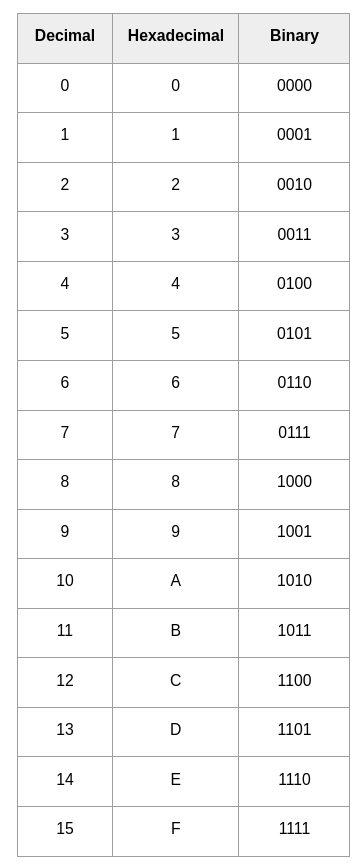
\includegraphics[width=5.0cm]{hex-chart.png}
		\end{center}
	
		\par\noindent \textbf{(II)} A string of 0's and 1's is difficult to read, so we will instead divide the binary string into segments of 4 bits. We can then use the table to replace each segment with the corresponding hexadecimal digit. Consider the string 000111000011:
		
		\begin{flalign*}
			(0001\;\;\;1100\;\;\;0011)_{2}  = (1\;\text{C}\;3)_{16}			
		\end{flalign*}
		
		\par\noindent 000111000011 and 1C3 are the binary and hexadecimal representations of 451, which we can verify:
		
	\end{minipage}	
	\hspace{0.45cm}
	\begin{minipage}[t]{.5\linewidth} 
		\par\noindent Binary Verification:
		\begin{flalign*}
			2^8+2^7+2^6+2^1+2^0 = 451
		\end{flalign*}
		\par\noindent Hexadecimal Verification:
		\begin{flalign*}
			(1)(16)^2 + (12)(16)^1 + (3)(16)^0 = 451
		\end{flalign*}
	
		\par\noindent\textbf{(III)} Let's try to rewrite the binary string 0100101111110101 using hexadecimals:
		 
		 \begin{flalign*}
		 	(0100\;\;\;1011\;\;\;1111\;\;\;0101)_2 = (4\;\text{B}\;\text{F}\;5)_{16}
		 \end{flalign*}
	 
	 	 \par\noindent We can see that both are representations of the decimal \(19445\). The hexadecimal verification is shown below:
	 	 \begin{flalign*}
	 	 	(4)(16)^3 + (11)(16)^2 + (15)(16)^1 + (5)(16)^0 \\ = 19445
	 	 \end{flalign*}
 	 
 	 	\par\noindent\textbf{(IV)} To convince ourselves that this technique works we can decompose 4BF5 in the following manner:
		
		\begin{flalign*}
		 \begin{tabular}{r}
	4\;\;0\;\;0\;\;0 \\ 
	+ B\;\;0\;\;0 \\
	+ F\;\;0 \\
	+ 5 \\
	\hline
	4\;\;B\;\;F\;\;5
\end{tabular}
		\end{flalign*}
	
		\par\noindent Let's calculate the decimal representation of each row:
		
		\begin{flalign*}
			(4)(16)^3 = 16384\\
			(11)(16)^2 = 2816 \\
			(15)(16)^1 = 240 \\
			(5)(16)^0 = 5
		\end{flalign*}
		
		\par\noindent Finally, we can see that adding all of these results give us the original decimal: \(16384 + 2816 + 240 + 5 = 19445\).
		
	\end{minipage}
	
\end{document}